
\documentclass[hide notes,intlimits,handout]{beamer}


\mode<presentation>
{
  \usetheme[headline,footline]{UAFshade}
  \setbeamercovered{transparent}
}

% load packages
\usepackage[english]{babel}
\usepackage[latin1]{inputenc}
\usepackage[T1]{fontenc}
\usepackage{multimedia,pgf}
\usepackage{lmodern}
\usepackage[amssymb]{SIunits}
\usepackage{hyperref}
\usepackage{natbib}
\bibliographystyle{andy}


% title page
\title[Glacier Dynamics] % (optional, use only with long paper titles)
{Mechanics and Thermodynamics of Glaciers}
\subtitle{Glaciers 617}


\author[Aschwanden] % (optional, use only with lots of authors)
{Andy Aschwanden}
% - Give the names in the same order as the appear in the paper.
% - Use the \inst{?} command only if the authors have different
%   affiliation.

\institute[ARSC] % (optional, but mostly needed)
{
  %
  Arctic Region Supercomputing Center\\
  University of Alaska Fairbanks, USA
}
% - Use the \inst command only if there are several affiliations.
% - Keep it simple, no one is interested in your street address.




\subject{Glaciers}

% define what is shown at the beginning of each section
\AtBeginSection[]
{
 \begin{frame}<beamer>
   \frametitle{Outline}
   \tableofcontents[currentsection,subsectionstyle=hide/hide/hide]
 \end{frame}
}

% define what is shown at the beginning of each subsection
% \AtBeginSubsection[]
% {
%  \begin{frame}<beamer>
%   \frametitle{Outline}
%    \tableofcontents[currentsection,currentsubsection]
%  \end{frame}
% }

\begin{document}

% insert titlepage
\begin{frame}
  \titlepage
\end{frame}

% insert TOC
\begin{frame}
 \frametitle{Outline}
 \tableofcontents[subsectionstyle=hide]
  %You might wish to add the option [pausesections]
\end{frame}

\section{Introduction}


%{
%\setbeamertemplate{headline}[default]
%\begin{frame}
%  \frametitle{Why}
%  The flow of glaciers and ice sheets is an interesting, non-trival problem in fluid dynamics
%\end{frame}
%} 

\begin{frame}[plain] % not in the handout
  \begin{figure}
    \pgfputat{\pgfxy(-.39,.25)}{
    \includegraphics<1| handout: 0>[width=\paperwidth]{figures/gorner}%
    \includegraphics<2>[width=\paperwidth]{figures/gorner_clarke}%    
  }
  \end{figure}
\end{frame}

\begin{frame}
  \frametitle{Ice Dynamics}
  unfortunately, \alert{ice dynamics} is
  \begin{itemize}
    \item physics
    \item continuum mechanics
    \item thermodynamics
    \item and equations, equations, and more equations
  \end{itemize}
\end{frame}

\begin{frame}
  \frametitle{Course Material}
  \begin{itemize}
    \item notation follows closely \cite{GreveBlatter_disg}
    \item covers parts of Chapters~3\,--\,5.1
    \item \url{http://www.gi.alaska.edu/~aaschwanden/lecture.html}
  \end{itemize}
  \def\newblock{}
  \bibliography{cryo}
\end{frame}



\begin{frame}
  \frametitle{Observations}
    \begin{block}{1779 Gravitation theory by de~Saussure}
      H.~B. de~Saussure observes sliding
      \begin{itemize}
        \item ``\ldots the weight of the ice might be sufficient to urge it down the slope of the valley, if the sliding motion were aided by the water flowing at the bottom.''
      \end{itemize}
    \end{block}
    \begin{block}{1827-1836 Hugi Block}
      J.~Hugi observed that a boulder moved $1315\,\text{m}$ downstream between 1827 and 1836
      \begin{itemize}
        \item we would interpret this as clear evidence of glacier flow
        \item but back then, some people argued that a boulder slids on the glacier surface, the glacier itself is motionless
      \end{itemize}
    \end{block}
\end{frame}

\begin{frame}
  \frametitle{Observations}
  \begin{figure}
    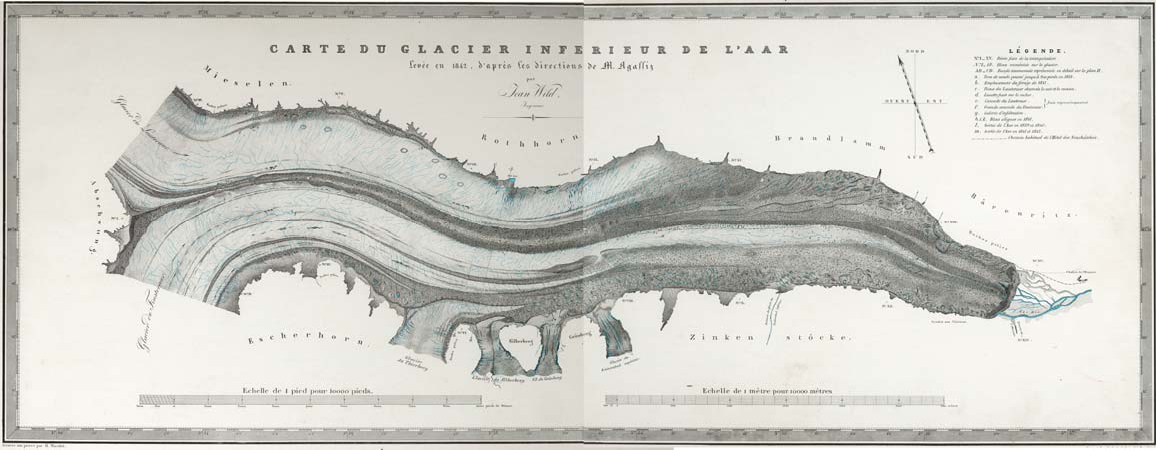
\includegraphics[width=8cm]{figures/agassi}%
  \end{figure}
    \begin{block}{1840-1846 Dilatation theory by L. Agassi}
      \begin{itemize}
        \item glacier ice contains innumerable fissures and capillary tubes
        \item during the day, these tubes absorb the water
        \item and during the night, the water freezes
        \item this distension exerts a force and propels the glacier in the direction of least resistance
      \end{itemize}
    \end{block}
\end{frame}



\begin{frame}
  \frametitle{Observations}
  \begin{columns}
    \column[C]{4.25cm}
    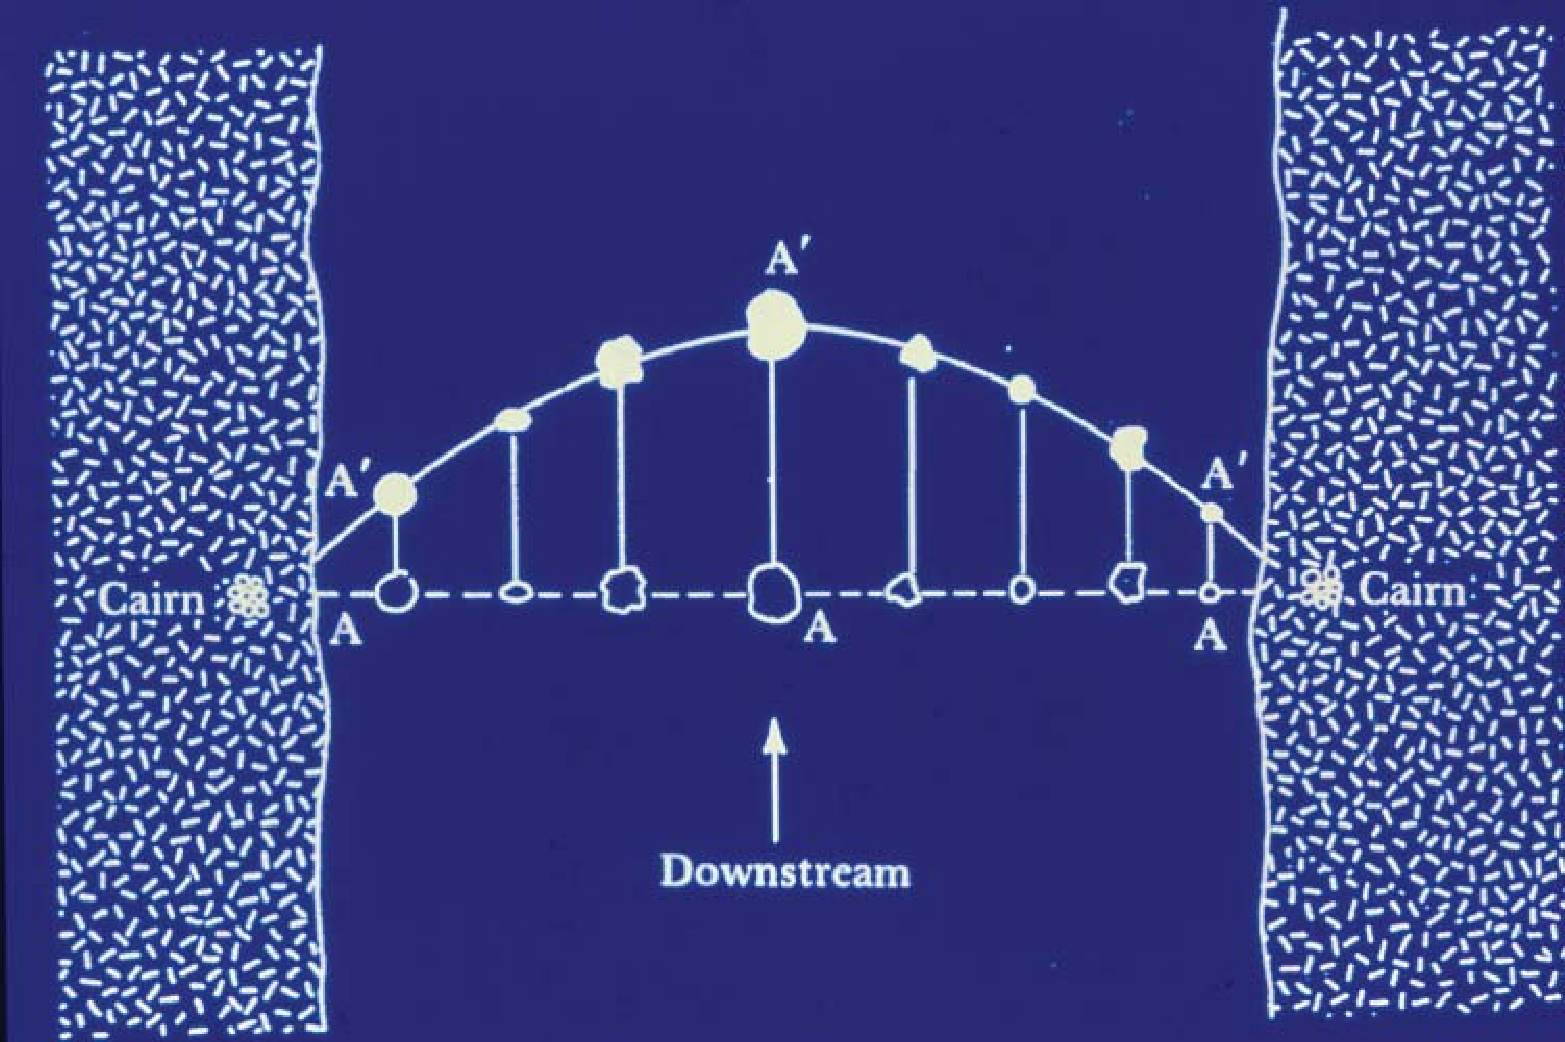
\includegraphics[width=4cm]{figures/geschw_prof_oberfl}%
    \vskip1em
    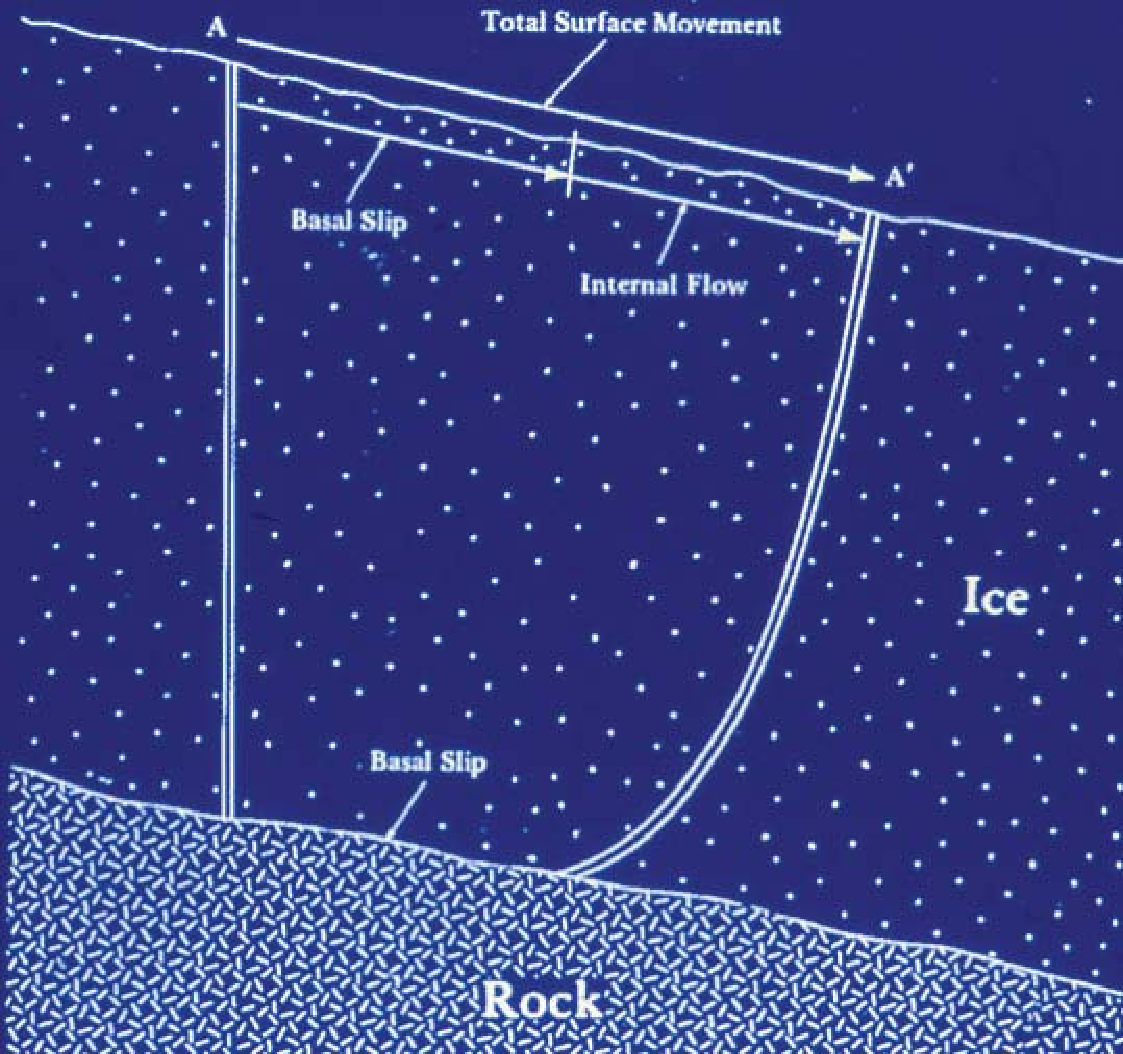
\includegraphics[width=4cm]{figures/geschw_vert_prof}%
    \column[C]{7.75cm}
    \begin{block}{1864-1930 Viscous flow theory by J.~Forbes}
      \begin{itemize}
        \item made his own observations on Mer de Glace, France
          \item glacier flows fastest in the center
        \item opposes Agassi's theory
        \item if the dilatation theory were true
        \item then flow would be greatest at sunset
        \item and near the glacier margins
      \end{itemize}
    \end{block}
 \end{columns}
\end{frame}

 
\begin{frame}
  \frametitle{Questions}
  \centering{
    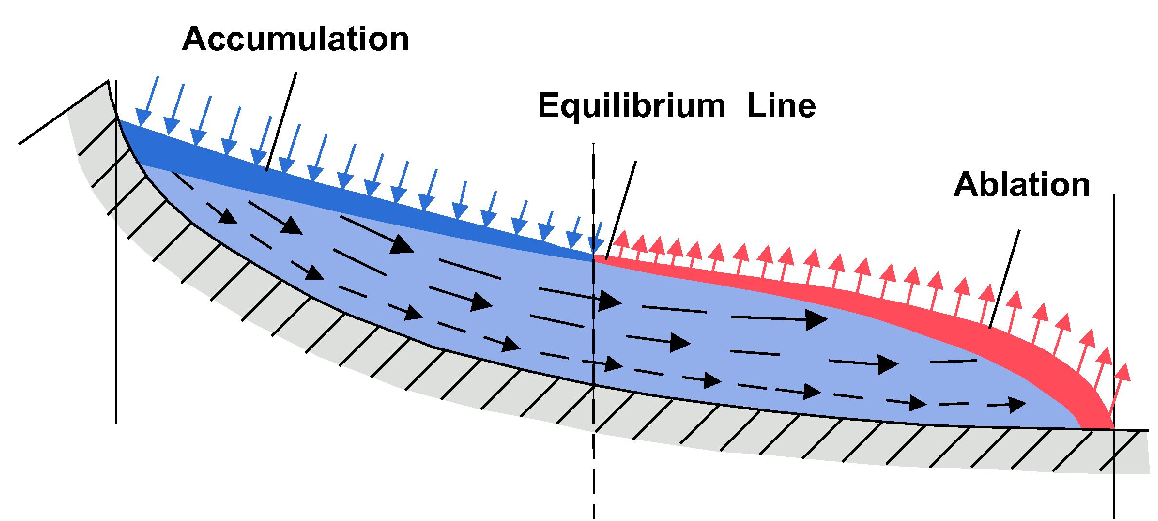
\includegraphics[width=.65\textwidth]{figures/flow_acc_abl}
  }
 \begin{itemize}
    \item What determines the glacier shape and extent
    \item How do ablation, accumulation, ice temperature, and the bedrock topography influence the flow of a glacier
    \item How does the flow speed vary with depth, along a flowline, or orthogonal to a flowline
  \end{itemize}
\end{frame}

\begin{frame}
  \frametitle{Questions}
  \centering{
    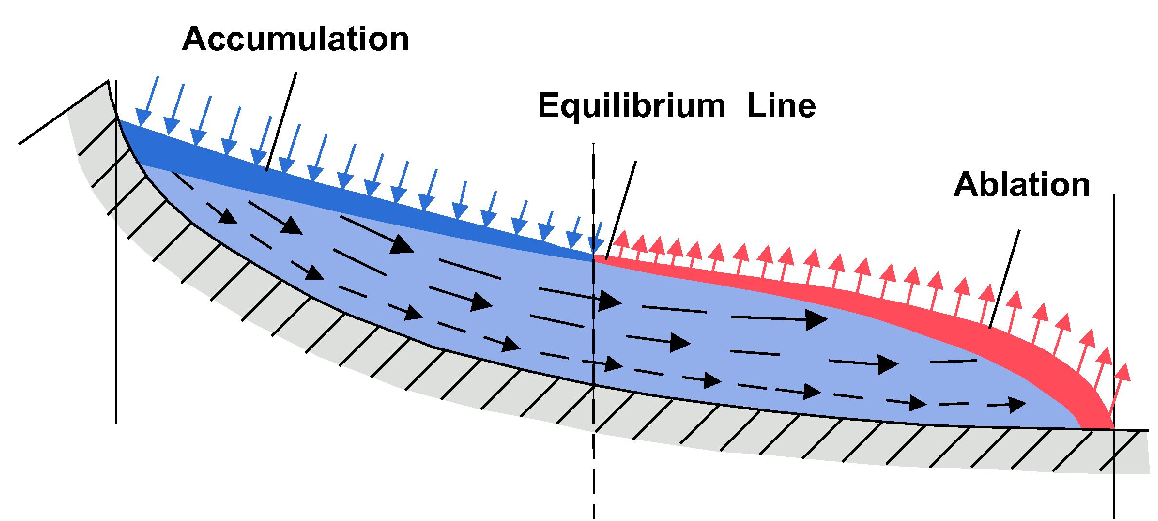
\includegraphics[width=.5\textwidth]{figures/flow_acc_abl}
  }
 \begin{block}{The two major problems}
   \begin{enumerate}
   \item Given the boundary conditions,
     \begin{itemize}
     \item basal topography
     \item accumulation-ablation function
     \item temperature at the upper ice surface
     \item geothermal heat flux at the base,
   \end{itemize}
   which glacier (geometry) is in equilibrium for given bc's.
  \item How does the glacier respond to changes in the bc's?
\end{enumerate}
  \end{block}
\end{frame}

\begin{frame}
  \frametitle{Answer}
  \centering{
    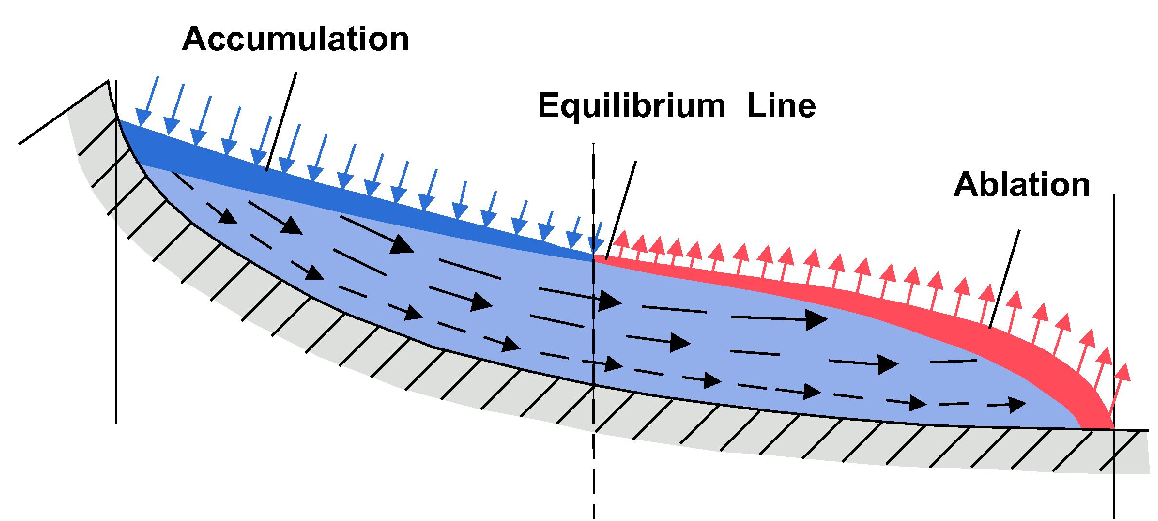
\includegraphics[width=.5\textwidth]{figures/flow_acc_abl}
  }

 \begin{block}{Solution: Continuum Mechanics \& Rheology}
   \begin{itemize}
     \item Solve balance equations for
       \begin{itemize}
       \item mass
       \item linear and angular momentum
       \item energy
       \item (forget about entropy)
       \end{itemize}
     \item Define constitutive equations
  \end{itemize}
  \note{useful stuff, not only for ice dynamics. recently applied by Truffer to solve a surface mass balance problem}
\end{block}
\end{frame}


\section{Balance Equations}

\begin{frame}
  \frametitle{General Balance Equations}
  \begin{block}{In integral form}
    \begin{eqnarray}
      \frac{\text{d} }{\text{d} t} \int_{\omega} g \, \text{d} v & = & - \oint_{\partial \omega} \boldsymbol{\phi} \cdot \mathbf{n} \, \text{d} a +  \int_{\omega} \left(p + s\right) \, \text{d} v \\
      & = & - \int_{\omega} \nabla \cdot \boldsymbol{\phi} \, \text{d} v +  \int_{\omega} \left(p + s\right) \, \text{d} v
    \end{eqnarray}
    \begin{columns}
      \column[C]{0.1cm}
      $g$ \\
      $\boldsymbol{\phi}$ \\
      $p$ \\
      $s$ \\
      \column[C]{6cm}
      physical quantity \\
      flux of $g$ through the boundary \\
      production of $g$ \\
      supply of $g$
    \end{columns}
  \end{block}

\end{frame}

\begin{frame}
  \frametitle{General Balance Equation}
  \begin{block}{In local form}
    \begin{equation}
      \frac{\partial g}{\partial t} = - \nabla \cdot \left(\boldsymbol{\phi} + g\mathbf{v}\right) + p + s
    \end{equation}
    \begin{columns}
      \column[C]{0.1cm}
      $g$ \\
      $\boldsymbol{\phi}$ \\
      $p$ \\
      $s$ \\
      \column[C]{6cm}
      physical quantity \\
      flux of $g$ through the boundary \\
      production of $g$ \\
      supply of $g$
    \end{columns}
  \end{block}
  use
  \begin{itemize}
    \item Reynolds transport theorem
    \item Divergence theorem
    \end{itemize}
    to go back and forth
\end{frame}


\subsection{Mass Balance}

\begin{frame}
  \frametitle{Mass Balance}
  \begin{itemize}
    \item the mass of a material volume cannot change, $\text{d} M/\text{d} t=0$
    \end{itemize}
    \begin{columns}
      \column[C]{1cm}
      $g = \rho$ \\
      $\boldsymbol{\phi} =0 $ \\
      $p = 0$ \\
      $s = 0$ \\
      \column[C]{6cm}
      mass density \\
      flux of $g$ through the boundary \\
      production of $g$ \\
      supply of $g$
    \end{columns}
    \vskip1em
    from the above we get
   \begin{equation}
      \frac{\text{d}}{\text{d} t} \int_{\omega} \rho \, \text{d} v = 0
    \end{equation} or in local form
    \begin{equation}
      \frac{\partial \rho}{\partial t} + \nabla \cdot \left(\rho \mathbf{v}\right) = 0
    \end{equation}
    $\Rightarrow$ known as the \alert{continuity equation}
\end{frame}


\subsection{Momentum Balance}

\begin{frame}
  \frametitle{Momentum Balance}
  Newton's Second Law
  \begin{itemize}
    \item total rate of change of momentum $\mathbf{P}$ equals sum of all forces $\mathbf{F}$
    \begin{equation}
      \frac{\text{d} \mathbf{P}}{\text{d} t} = \mathbf{F} = \underbrace{\oint_{\partial \omega} \mathbf{t}_{\mathbf{n}} \, \text{d} a}_{\text{internal}} +\underbrace{\int_{\omega} \mathbf{f} \, \text{d} v}_{\text{external}}
    \end{equation}
  \item identify $\mathbf{t}_{\mathbf{n}} = \mathbf{T}\mathbf{n}$
  \item $\mathbf{T}$ is the \alert{Cauchy stress tensor}
  \item external forces: gravity, Coriolis force,
  \end{itemize}    
\end{frame}


\begin{frame}
  \frametitle{Momentum Balance}
  from the previous we get
  \begin{eqnarray}
    \frac{\text{d}}{\text{d} t} \int_{\omega} \rho \mathbf{v}\, \text{d} v & = & - \oint_{\partial \omega} \mathbf{T} \cdot \mathbf{n} \, \text{d} a + \int_{\omega} \mathbf{f} \, \text{d} v \\
    & & -\int_{\omega} \nabla \cdot \mathbf{T}\, \text{d} v + \int_{\omega} \mathbf{f} \, \text{d} v
  \end{eqnarray} or in local form
  \begin{equation}
    \frac{\text{d}\left(\rho\mathbf{v}\right)}{\text{d} t} = -\nabla \cdot \mathbf{T} + \mathbf{f}
  \end{equation}
  \begin{columns}
    \column[C]{2cm}
    $g = \rho \mathbf{v}$ \\
    $\boldsymbol{\phi} = - \mathbf{T} $ \\
    $p = 0$ \\
    $s = \mathbf{f}$ \\
    \column[C]{6cm}
      momentum density \\
      flux of $g$ through the boundary \\
      production of $g$ \\
      supply of $g$
    \end{columns}
\end{frame}


\subsection{Angular Momentum Balance}

\begin{frame}
  \frametitle{Angular Momentum Balance}
  \begin{itemize}
  \item  no, I don't want to do the whole derivation here
  \item if you're interested (or bored), go through Equations~3.77\,--\,3.83  in \cite{GreveBlatter_disg}
  \item here, we just use the result
  \item the stress tensor $\mathbf{T}$ is \alert{symmetric}
  \end{itemize}
  \begin{equation}
    \mathbf{T} = \mathbf{T}^{T}
 \end{equation}
\end{frame}


\subsection{Energy Balance}

\begin{frame}
  \frametitle{Energy Balance}
  \begin{itemize}
  \item  only the total energy (sum of kinetic and inner energy) is a \alert{conserved} quantity
  \item balance of kinetic energy is \alert{not an independent statement} but a mere consequence of the momentum balance
  \item here, we formulate the balance of specific inner energy, $u$:
  \end{itemize}
  \begin{equation}
    \rho\frac{\text{d} u}{\text{d} t} = - \nabla \cdot \mathbf{q} + \text{tr}\left(\mathbf{T}\cdot\mathbf{D}\right) + \rho r
  \end{equation}
\vskip1em
 \begin{columns}
   \column[C]{3cm}
   $g = u$ \\
   $\boldsymbol{\phi} = \mathbf{q} $ \\
   $p = \text{tr}\left(\mathbf{T}\cdot\mathbf{D}\right) $ \\
   $s = \rho r$ \\
   $\mathbf{D} = 1/2\left(\mathbf{v}^{T}+\mathbf{v}\right)$
   \column[C]{6cm}
   specific internal energy \\
   heat flux \\
   dissipation power \\
   specific radiation power\\
   \alert{strain rate} or \alert{velocity gradient} tensor
 \end{columns}
\end{frame}



\begin{frame}
  \frametitle{Balance Equations}
  \begin{equation*}
  \begin{array}{lcclc}
    \text{mass} \quad &  \frac{\text{d} \rho}{\text{d} t} & = & -\rho\nabla \cdot \mathbf{v} \quad & (1)\\[.25em]
    \text{momentum} \quad & \rho \frac{\text{d} \mathbf{v}}{\text{d} t} & = & -\nabla \cdot \mathbf{T} + \mathbf{f} \quad & (3) \\[.25em]
    \text{internal energy} \quad & \rho\frac{\text{d} u}{\text{d} t} & = & - \nabla \cdot \mathbf{q} + \text{tr} \left(\mathbf{T}\cdot\mathbf{D}\right) + \rho r\quad & (1)
  \end{array}
  \end{equation*}
\centering{
 \begin{columns}
   \column[T]{4cm} \centering{
   left-hand side \\
   $\rho$ (1)\\
   $\mathbf{v}$ (3)\\
   $u$ (1)
   }
   \column[T]{4cm} \centering{
   right-hand side \\
   $\mathbf{T}$ (6)\\
   $\mathbf{q}$ (3)
  }
 \end{columns}
  }
  \begin{itemize}
   \item so we have 5 equations for 14 unknown fields
   \item the system is highly under-determined
   \item[$\Rightarrow$] \alert{closure relations} required
 \end{itemize}
\end{frame}



\begin{frame}
  \frametitle{Closure Relations}
  \begin{itemize}
    \item \alert{balance equations} are universally valid
    \item \alert{closure relations} describe the specific behavior of a material
    \item \alert{closure relations} are often called \alert{constitutive equations}
  \end{itemize}
\end{frame}


\section{Constitutive Equations}

\subsection{Material Science}



\begin{frame}
  \frametitle{Material Science}
  \begin{block}{Rheology}
    \begin{itemize}
    \item is the study of the flow of complex liquids or the deformation of soft solids.
    \item We are not going through this in great detail.
    \item[$\Rightarrow$] For further information, consult the handout or
      \item take Martin Truffers ``Ice Physics 614''  class
    \end{itemize}
  \end{block}
  \begin{block}{We need to define}
    \begin{itemize}
    \item a constitutive equation for the heat flux $\mathbf{q}$
    \item and for the internal energy $u$
    \item a relationship between stress and strain, $\mathbf{T} = f(\mathbf{D})$
   \end{itemize}
  \end{block}
\end{frame}


\begin{frame}
  \frametitle{Rheology}
  \begin{itemize}
    \item ask a material scientist or rheologist
    \item and let him/her do some fancy experiments
 \end{itemize}
  \begin{figure}
  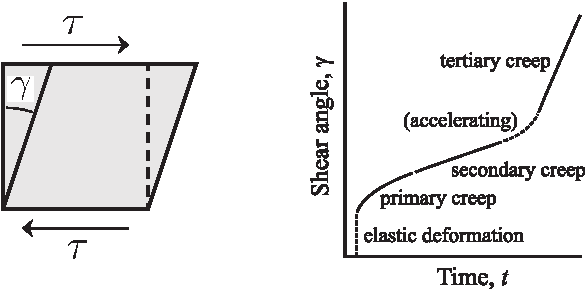
\includegraphics[width=7cm]{figures/fig_4_04}
  \end{figure}
  \note{
    apply a constant stress (creep experiment)
    \begin{itemize}
    \item if the material, after some deformation, eventually resists further deformation, it is a \alert{solid}
    \item if the material flows idefinitively, it's a \alert{liquid}
    \end{itemize}
  }
\end{frame}

\subsection{Shear Experiment}

\begin{frame}
  \frametitle{Example: Shear Experiment}
  \begin{itemize}
    \item apply constant shear stress $\boldsymbol{\tau}$
\end{itemize}
  \begin{columns}
    \column[c]{8cm}
    \begin{figure}
      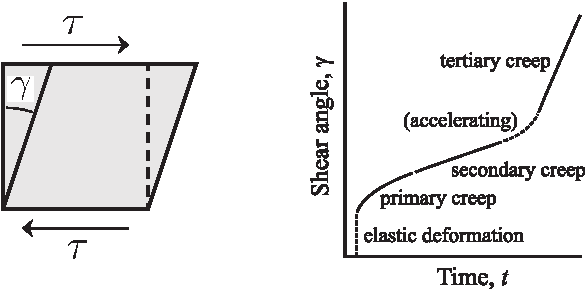
\includegraphics[width=6cm]{figures/fig_4_04}
    \end{figure}
    \column[c]{5cm}
    $\tau$ is the applied shear stress\\
    $\gamma$ is the shear angle\\
    $\dot\gamma$ is the shear rate
  \end{columns}
  \begin{itemize}
    \item initial elastic deformation
    \item primary creep: shear rate $\dot\gamma$ decreases with time
    \item \alert{secondary creep}: shear rate remains constant
    \item acceleration phase
    \item tertiary creep: constant shear rate (but higher) 
 \end{itemize}
\end{frame}


\begin{frame}
  \frametitle{Example: Shear Experiment}
  \begin{columns}
    \column[c]{8cm}
    \begin{figure}
      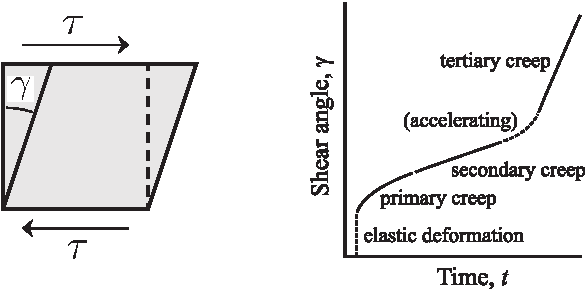
\includegraphics[width=6cm]{figures/fig_4_04}
    \end{figure}
    \column[c]{5cm}
    $\tau$ is the applied shear stress\\
    $\gamma$ is the shear angle\\
    $\dot\gamma$ is the shear rate
  \end{columns}
  \vskip1em
  This suggests that
  \begin{itemize}
  \item the shear rate is a function of the applied shear stress, temperature $T$, and pressure $p$
    \begin{equation}
      \dot\gamma = \dot\gamma\left(\tau,T,p\right)
    \end{equation}
   \end{itemize}
 \end{frame}


\begin{frame}
  \frametitle{Example: Shear Experiment}
  \begin{columns}
    \column[c]{8cm}
    \begin{figure}
      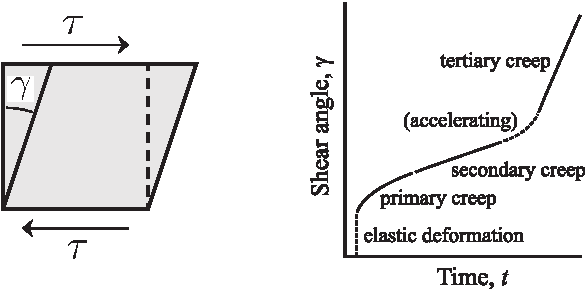
\includegraphics[width=6cm]{figures/fig_4_04}
    \end{figure}
    \column[c]{5cm}
    $\tau$ is the applied shear stress\\
    $\gamma$ is the shear angle\\
    $\dot\gamma$ is the shear rate
  \end{columns}
  \vskip1em
  \begin{itemize}
  \item The dynamic viscosity $\eta$ relates shear stress and shear rate
    \begin{equation}
      \tau = \eta\left(T,p,\vert \dot\gamma \vert\right)\dot\gamma
    \end{equation}
  \end{itemize}
\end{frame}


\subsection{Flow Relation}

\begin{frame}
  \frametitle{Generalization}
  \begin{block}{Assume}
  \begin{itemize}
  \item secondary creep
  \item incompressibility of ice, $\mathbf{T} = \underbrace{-p\mathbf{I}}_{\text{isotropic}} + \underbrace{\mathbf{T}'}_{\text{deviatoric}}$
\item with the pressure $p=-1/3\text{tr}{\mathbf{T}}$
  \end{itemize}
\end{block}
  \vskip.5em
  The only non-straightforward step from
  \begin{equation}
    \tau = \eta\left(T,p,\vert \dot\gamma \vert\right)\dot\gamma
  \end{equation}
  to
  \begin{equation}
    \mathbf{T}' = \eta\left(T,p,\vert \bullet \vert\right)\mathbf{D}
  \end{equation}
  is the generalization of $\vert \dot\gamma\vert$
\end{frame}

\begin{frame}
  \frametitle{Generalization}
  \begin{equation}
    \mathbf{T} = \eta\left(T,p,\vert \bullet \vert\right)\mathbf{D}
  \end{equation}
  is a relation between two tensors (i.e. $\mathbf{T}$ and $\mathbf{D}$)
  \begin{itemize}
  \item \alert{material objectivity} tells us that such a relationship must be independent of the chosen vector basis
  \item a second rank tensor has 3 scalar invariants
    \begin{eqnarray}
      I_{\mathbf{T}'} & = & \text{tr}\mathbf{T}' \\
      II_{\mathbf{T}'} & = & 1/2\left(\left(\text{tr}\mathbf{T}'\right)^{2}  -\text{tr}\left(\mathbf{T}'\right)^{2}\right)\\
      III_{\mathbf{T}'} & = & \text{det}\,\mathbf{T}'
    \end{eqnarray}
    \item $\text{tr}\mathbf{T}'=0$ for incompressible media
    \item $\sigma_{\text{e}} = \sqrt{II_{\mathbf{T}'}}$ is the \alert{effective stress}
    \item role of $ III_{\mathbf{T}'}$ is not clear, but lab experiments indicate that the third invariant is not important
  \end{itemize}
\end{frame}

\begin{frame}
  \frametitle{Generalization}
  Numerous lab experiments and field measurements suggest
    \begin{equation}
      \frac{1}{\eta\left(T,p,\sigma_{\text{e}}\right)} =2A\left(T,p\right)f\left(\sigma_{\text{e}}\right)
    \end{equation}
    where
    \begin{equation*}
      \begin{array}{rcll}
      A(T,p) & = & A_{0} e^{-(Q+pV)/T} &\qquad \text{Arrehenius law}\\[.25em]
      f\left(\sigma_{\text{e}}\right) & = &\sigma_{\text{e}}^{n-1} &\qquad \text{power law}
      \end{array}
    \end{equation*}
    \vskip1em
    This is known as \alert{Glen's flow law} or \alert{Glen-Steinemann flow law}
\end{frame}

\begin{frame}
  \frametitle{Calorimetric Equation of State}
  Internal energy, $u$ depends linearly on temperature, $T$,
  \begin{equation}
    u = u_{0} + c\left(T-T_{0}\right)
  \end{equation}
  where $u_{0}$ is a reference value at a reference temperature $T$
\end{frame}

\begin{frame}
  \frametitle{Heat Flux}
 \begin{block}{Fourier Equation}
  \begin{columns}
    \column[c]{5.5cm}
  \begin{figure}
    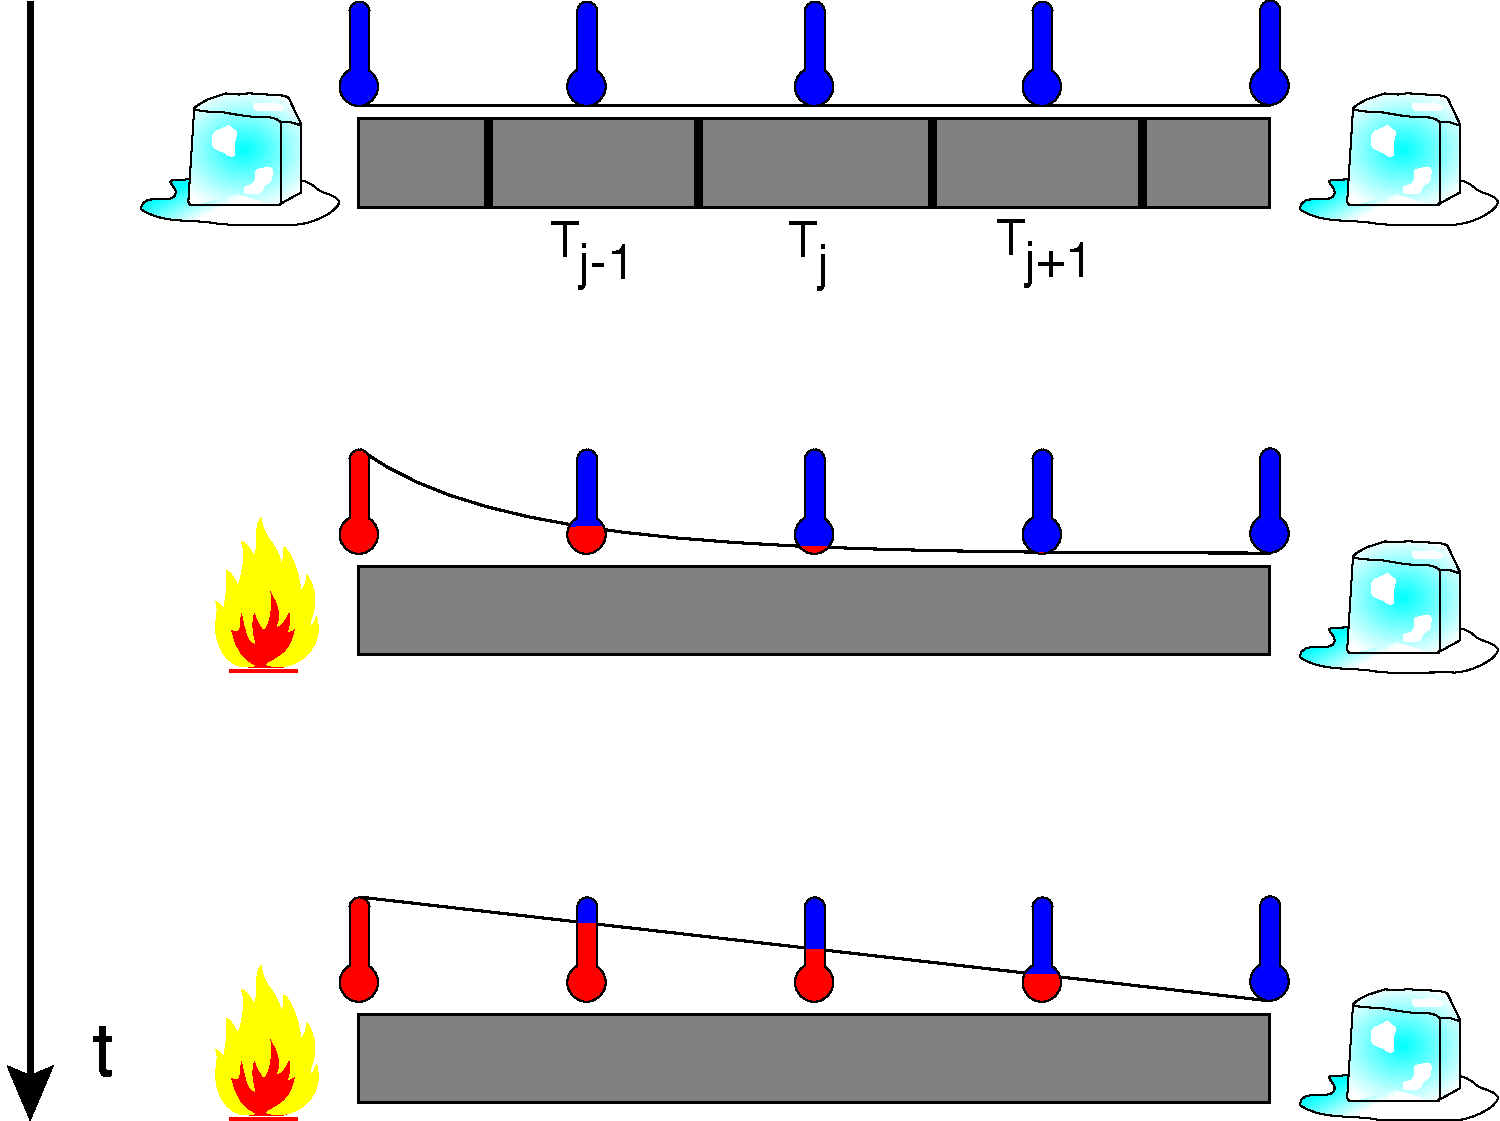
\includegraphics[width=5cm]{figures/heatconduction}%
   \\[.25em] \tiny{modified after \emph{Christophe Dang Ngoc Chan, wiki commons image}}
  \end{figure} 
    \column[c]{6.5cm}
  \begin{itemize}
  \item heat flows from \alert{higher} to \alert{lower} temperature
 \begin{equation*}
    \mathbf{q} = -k \nabla T
  \end{equation*}
  \item the thermal conductivity $k$ is a measure for how fast the heat spreads
 \end{itemize}
  \end{columns}
\end{block}
\end{frame}


\section{Glaciers}


\begin{frame}
  \frametitle{Large-Scale Dynamics}
  \begin{figure}
    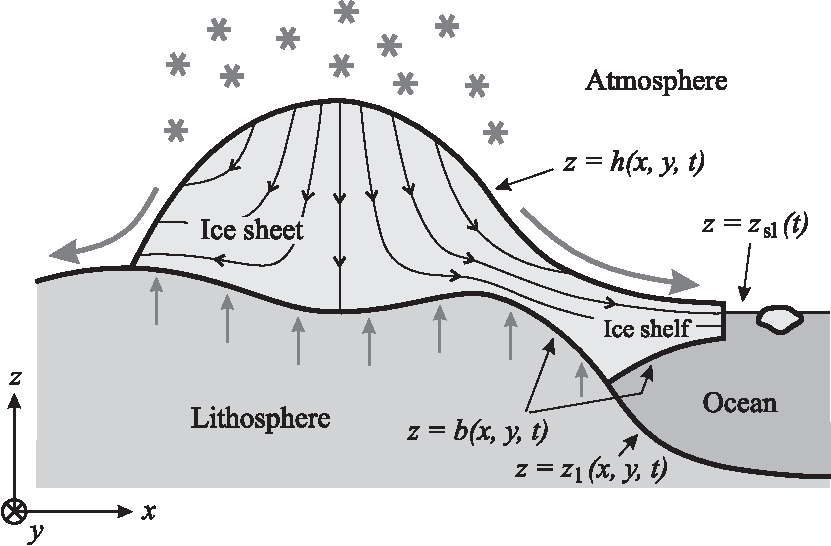
\includegraphics[width=.55\textwidth]{figures/fig_5_01}%
  \end{figure}
 \begin{itemize}
    \item Ice sheets are glaciers too!
      \item ice is assumed to be incompressible, $\nabla \cdot \mathbf{v} = 0$
  \end{itemize}
\end{frame}

\begin{frame}
  \frametitle{Recap}
  \begin{block}{Balance Equations}
    \begin{equation*}
      \begin{array}{lrclc}
        \text{mass} \quad &  0& = & \nabla \cdot \mathbf{v} \quad & (1)\\[.25em]
        \text{momentum} \quad & \rho \frac{\text{d} \mathbf{v}}{\text{d} t} & = & -\nabla \cdot \mathbf{T'} + \nabla p + \mathbf{f} \quad & (3) \\[.25em]
        \text{internal energy} \quad & \rho\frac{\text{d} u}{\text{d} t} & = & - \nabla \cdot \mathbf{q} + \text{tr} \left(\mathbf{T}\cdot\mathbf{D}\right) + \rho r\quad & (1)
      \end{array}
    \end{equation*}
  \end{block}
  \begin{block}{Flow Law}
    \begin{equation*}
      \begin{array}{lrclc}
              \text{Glen's flow law}\quad & \mathbf{T}' & = & 2\,\eta\,\mathbf{D}  = 1/2 A^{-1/n}\varepsilon_{\text{e}}^{\frac{1-n}{n}} \mathbf{D} \quad &(6)
      \end{array}
    \end{equation*}
  \end{block}
  \begin{itemize}
  \item now we have 15 equations for 15 unknown fields, $\rho (1), \mathbf{v} (3), p (1), \mathbf{T}' (6), u (1), \mathbf{q} (3)$
   \item the system is still under-determined, but we are getting closer
   \end{itemize}
 \end{frame}
 
 
\subsection{Scale analysis}

\begin{frame}
  \frametitle{The Big Picture}
  \begin{block}{Momentum Balance}
    \begin{equation}
        \rho \frac{\text{d} \mathbf{v}}{\text{d} t} = -\nabla \cdot \mathbf{T'} + \nabla p + \underbrace{\rho\mathbf{g}}_{\text{gravity}} - \underbrace{2\rho\boldsymbol{\Omega} \times \mathbf{v}}_{\text{Coriolis force}} 
   \end{equation}
   This is the \alert{Navier-Stokes} equation for incompressible flow
  \end{block}
  \begin{block}{Flow Law}
    \begin{equation}
      \begin{array}{lrclc}
              \text{Glen's flow law}\quad & \mathbf{T}' & = & 2\,\eta\,\mathbf{D}  = 1/2 A^{-1/n}\varepsilon_{\text{e}}^{\frac{1-n}{n}} \mathbf{D} \quad &(6)
      \end{array}
    \end{equation}
  \end{block}
  \begin{itemize}
  \item now we have 15 equations for 15 unknown fields, $\rho (1), \mathbf{v} (3), p (1), \mathbf{T}' (6), u (1), \mathbf{q} (3)$
   \item the system is still under-determined, but we are getting closer
   \end{itemize}
 \end{frame}
 

\begin{frame}
  \frametitle{Scale Analysis}
  \begin{block}{Some typical values for an ice sheet}
  \begin{equation*}
  \begin{array}{rccl}
    \text{horizontal extend} &  [L] & = & \unit{1000}\kilo\meter\\
    \text{vertical extend} & [H] & = & \unit{1}\kilo\meter \\
    \text{horizontal velocity} & [U] & = & \unit{100}\meter\power{a}{-1}\\
    \text{vertical velocity} & [W] & = & \unit{0.1}\meter\power{a}{-1}\\
    \text{pressure} & [U] & = & \rho g[H] = \unit{10}\mega\pascal\\
    \text{time-scale} & [T] & = &[L]/[U] = 10^{4}\usk\power{a}{1}\\
  \end{array}
  \end{equation*}
  \end{block}
  The aspect ratio $\epsilon$ is defined as
  \begin{equation*}
    \epsilon = \frac{[H]}{[L]} = \frac{[U]}{[W]} = 10^{-3} \text{ for an ice sheet}
  \end{equation*}
  \begin{itemize}
    \item The scaling argument for valley glaciers is almost the same
  \end{itemize}
\end{frame}


\begin{frame}
  \frametitle{Scale Analysis}
  \begin{block}{Froude number}
    The \alert{Froude number $Fr$} is the ratio of acceleration and pressure gradient. In the horizontal we have
  \begin{equation*}
    Fr = \frac{\rho[U]/[t]}{[P]/[L]} = \frac{\rho[U]^{2}/[L]}{\rho g [H]/[L]} = \frac{[U]^{2}}{g[H]} \approx 10^{-15}
  \end{equation*}
  and in the vertical
  \begin{equation*}
    Fr = \frac{\rho[W]/[t]}{[P]/[L]} = \frac{\rho[W]^{2}/[L]}{\rho g [H]/[L]} = \frac{[\epsilon U]^{2}}{g[H]} \approx 10^{-21}
  \end{equation*}
  $\Rightarrow$ The \alert{acceleration term} is \alert{negligible}
  \end{block}
\end{frame}


\begin{frame}
  \frametitle{Scale Analysis}
  \begin{block}{Rossby number}
    The \alert{Rossby number $Ro$} is the ratio of acceleration and Coriolis force
  \begin{equation*}
    Ro = \frac{[U]}{\Omega [L]} \approx 2\times10^{-8}
  \end{equation*}
  and thus the Coriolis to pressure gradient is
  \begin{equation*}
   \frac{Fr}{Ro}\approx 10^{-8}
  \end{equation*}
  $\Rightarrow$ The \alert{Coriolis term} is also \alert{negligible}
  \end{block}
\end{frame}


\subsection{Stokes Equation}


\begin{frame}
  \frametitle{Stokes Equation}
  By neglecting both the
  \begin{itemize}
  \item acceleration term
  \item Coriolis term
  \end{itemize}
  the Navier-Stokes equation simplifies to
  \begin{eqnarray}
     \nabla \cdot \left(\eta\left(\nabla \mathbf{v} + \nabla \mathbf{v}^{\text{T}}\right)\right) - \nabla p & = & - \rho \mathbf{g}
  \end{eqnarray}
  \begin{itemize}
  \item gravitational force exerted on the ice is balanced by stress within the ice
  \item this is called the \alert{Stokes equation}
  \end{itemize}
\end{frame}


\subsection{Energy Balance}

\begin{frame}
  \frametitle{Specific Internal Energy}
  Recall the balance equation for specific inner energy
  \begin{equation}
    \rho\frac{\text{d} u}{\text{d} t} = - \nabla \cdot \mathbf{q} + \text{tr} \left(\mathbf{T}\cdot\mathbf{D}\right) + \rho r
  \end{equation}
  \begin{itemize}
  \item radiation is negligible
 \end{itemize}
  \begin{equation}
    \rho\frac{\text{d} u}{\text{d} t} = - \nabla \cdot \mathbf{q} + \text{tr} \left(\mathbf{T}\cdot\mathbf{D}\right)
  \end{equation}
\end{frame}



\subsection{Boundary Conditions}


\begin{frame}
  \frametitle{Free Surface}
  
\end{frame}


\section{Math Stuff}

\begin{frame}
  \frametitle{Recall from Vector Calculus}
  \vskip-.25em
  \begin{block}{Divergence Theorem}
    \begin{equation}
      \oint_{\partial \omega} \boldsymbol{\phi} \,\text{d}a = 
      \int_{\omega} \nabla \cdot \boldsymbol{\phi} \, \text{d} v
    \end{equation}
      \begin{itemize}
      \item The sum of all sources minus the sum of all sinks gives the net flow out of a region
     \end{itemize}
  \end{block}
  \begin{block}{Reynolds Transport Theorem}
    \begin{equation}
     \frac{\text{d}}{\text{d} t}\int_{\omega} \boldsymbol{\phi}\, \text{d} v =
     \int_{\omega} \frac{\partial \boldsymbol{\phi}}{\partial{t}} \, \text{d} v +
      \oint_{\partial \omega} \boldsymbol{\phi} \mathbf{v}\cdot\mathbf{n}\,\text{d}a 
    \end{equation}
      \begin{itemize}
     \item What was already there plus what goes in minus what goes out is what is there
      \end{itemize}
  \end{block}
\end{frame}


\begin{frame}
  \frametitle{The Cauchy Stress Tensor}
  \begin{columns}
    \column[c]{6cm}
    \begin{figure}
      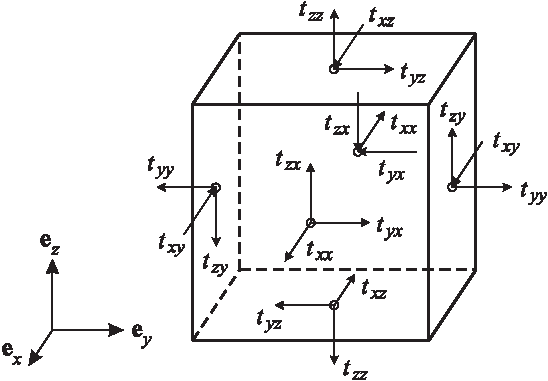
\includegraphics[width=5.cm]{figures/fig_3_08}
    \end{figure}
    \column[c]{5cm}
  \begin{displaymath} 
    \mathbf{T} = \left( 
      \begin{array}{ccc} 
        t_{xx} & t_{xy} & t_{xz} \\ 
        t_{yx} & t_{yy} & t_{yz} \\ 
        t_{zx} & t_{zx} & t_{zz} 
      \end{array} 
    \right) 
  \end{displaymath}
  \end{columns}
  \vskip1em
  For example
  \begin{displaymath}
    \mathbf{t}_{\mathbf{e}_{z}} =
    \left(
      \begin{array}{c}
        t_{xz}\\
        t_{yz}\\
        t_{zz}
      \end{array}
    \right)
  \end{displaymath}
  is the stress vector of a cut along the xy-plane
\end{frame}

\end{document}


